\section{Proposed solutions}

\begin{frame}{Proposed solutions}

    One of the most evident cause of instability and inaccuracy in CSACs is the Doppler broadening of the atomic transitions and the collisional shifts happening in the reference cell.

    \vspace{10pt}

    To reduce these effect and improving clock performances, three possible solutions are being investigated:

    \begin{itemize}
        \item Microwave transitions in a laser-cooled alkali metals
        \item Microwave transitions in double-resonance trapped ions
        \item Optical transitions in warm atomic/molecular vapors
    \end{itemize}

\end{frame}

\section*{Microwave transitions in laser-cooled alkali metals}

\begin{frame}{Working principle}

    Atoms cooling is a common technique used to \textbf{mitigate the Doppler broadening} of the atomic transitions and \textbf{reduce the collisional shifts}.

    \begin{figure}
        \centering
        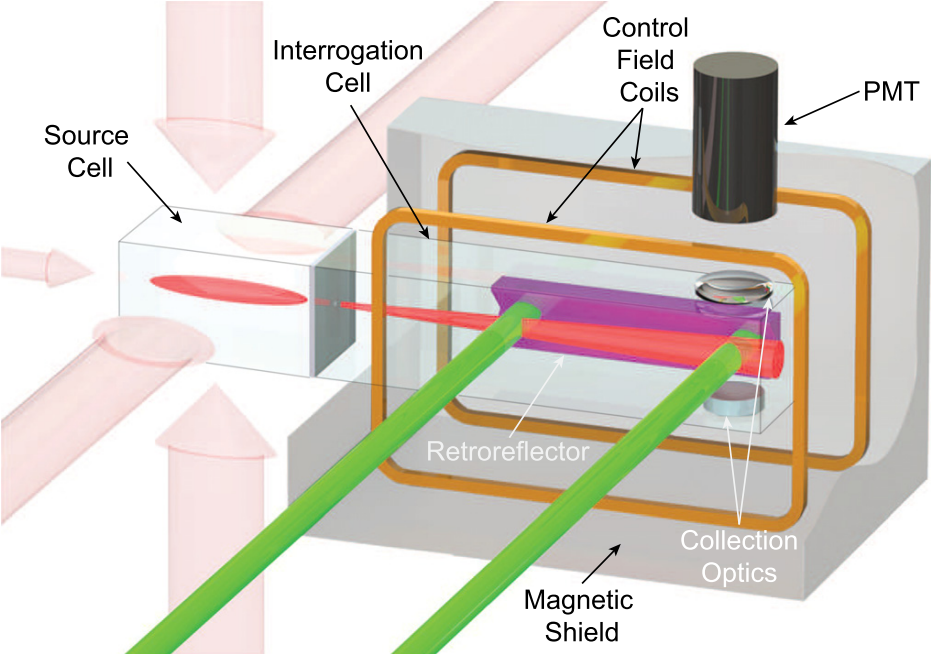
\includegraphics[width=0.6\textwidth]{img/laser-cooled-alkali-metals-trapping.png}
        \caption{Schematic of a 2D-MOT\footnotemark[1] and the interrogation cell.}
    \end{figure}

    \footnotetext[1]{2D-MOT: 2D Magneto-Optical Trap}
    \footnotetext[2]{PMT: Photo-Multiplier Tube}

\end{frame}



\begin{frame}{Current results}

    Stability results look promising but as of today the main bottlenecks are given by the \textbf{technological and experimental limitations}.
    A consistent advancement in those areas is needed to make this technology a viable solution for the future.

    \begin{columns}[T, onlytextwidth]

        \begin{column}{0.5\textwidth}

            \begin{figure}
                \centering
                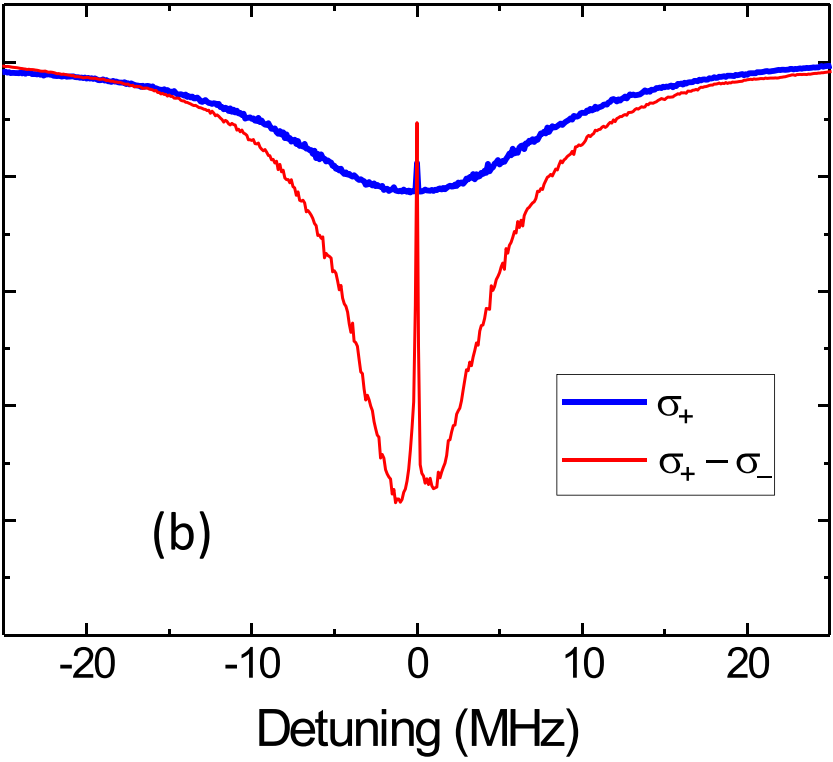
\includegraphics[height=0.45\textheight]{img/laser-cooled-alkali-metals-trasmission.png}
                \caption{\textcolor[HTML]{CA0200}{Laser-cooled} vs. \textcolor[HTML]{3700A7}{traditional} CSAC transmission.}
            \end{figure}

        \end{column}

        \begin{column}{0.5\textwidth}

            \begin{figure}
                \centering
                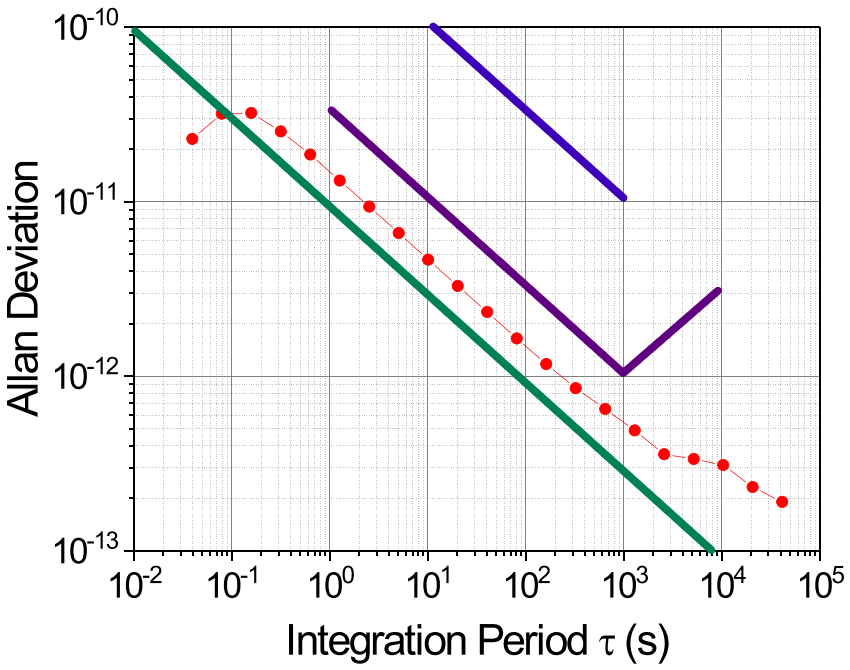
\includegraphics[height=0.45\textheight]{img/laser-cooled-alkali-metals-stability.png}
                \caption{
                    \textcolor[HTML]{006C43}{Target},
                    \textcolor[HTML]{4C0062}{SA.55 MAC},
                    \textcolor[HTML]{3700A7}{SA.45s CSAC},
                    \textcolor[HTML]{CA0200}{Laser-cooled CSAC}
                }
            \end{figure}

        \end{column}

    \end{columns}

\end{frame}
\section*{Microwave transitions in double-resonance trapped ions}

\begin{frame}{Working principle}

    The working principle is very similar to the one of the laser-cooled alkali metals, but with the \textbf{use of ions instead of atoms and a different cooling mechanism}.

    \begin{figure}
        \centering
        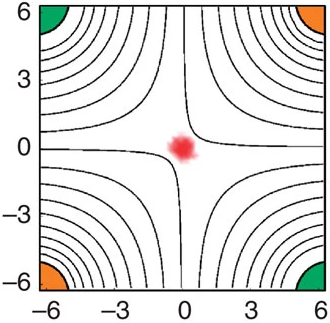
\includegraphics[height=0.35\textheight]{img/Paul-trapping-1.png}
        \hfill
        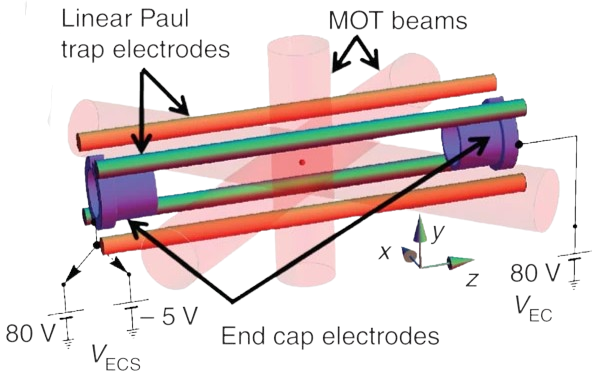
\includegraphics[height=0.35\textheight]{img/Paul-trapping-2.png}
        \caption{Schematic of the ion trapping setup (Paul trap).}
    \end{figure}

    The strong reduction of the Doppler broadening and the possibility of miniaturization makes this approach the most favorable for the NG-CSACs.

    \footnotetext[1]{MOT: Magneto-Optical Trap}

\end{frame}



\begin{frame}{Ytterbium based clock}

    \begin{columns}[c, onlytextwidth]

        \begin{column}{0.31\textwidth}

            \begin{figure}
                \centering
                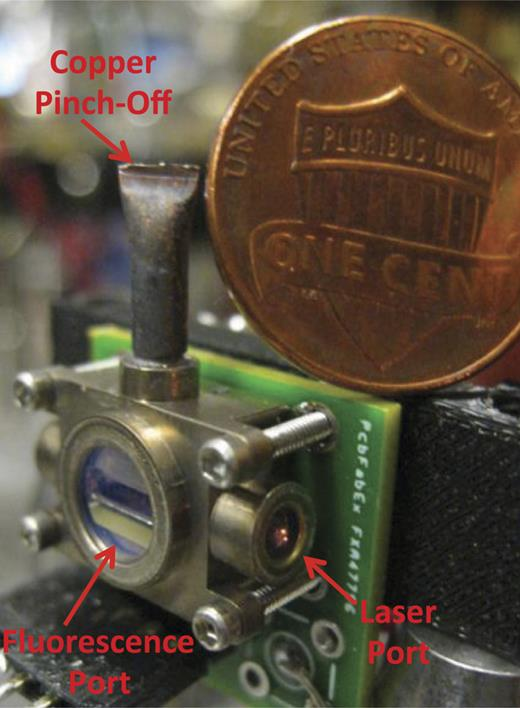
\includegraphics[width=\textwidth]{img/Ytterbium-clock.jpeg}
                \caption{Ion trap and vacuum package ($\approx 0.8cm^3$).}
            \end{figure}

        \end{column}

        \hfill

        \begin{column}{0.65\textwidth}

            One example of this technology is the $^{171}Yb^+$-based clock, \textbf{developed by Sandia and JPL (2015)}.

            \vspace{10pt}

            Known challenges and complications to achieve higher performances are:

            \begin{itemize}
                \item Stark Shift effect\footnotemark[1]: pulsed laser interrogation is required to avoid a shift in the ions transition frequency.
                \item Long life state $^2F_{7/2}$: the ions can fall into a long life state, from which must be released used an additional laser source or buffer gas.
            \end{itemize}

        \end{column}

    \end{columns}

    \footnotetext[1]{Start Shift effect: dependence of the atomic energy levels on the applied electric field.}

\end{frame}



\begin{frame}{Mercury based clock}

    Another example is the $^{199}Hg^+$-based clock, \textbf{developed by JPL (2019)} as a miniaturization of the current Deep Space Atomic Clock (DSAC).

    \vspace{10pt}

    \begin{columns}[c, onlytextwidth]

        \begin{column}{0.4\textwidth}

            \begin{figure}
                \centering
                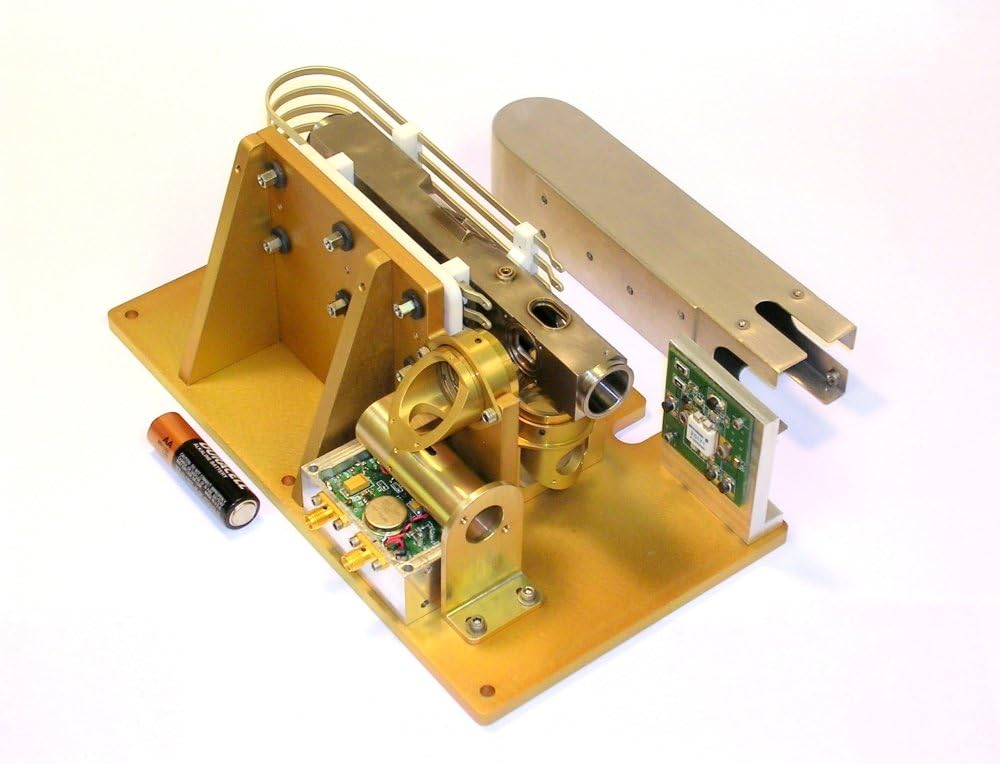
\includegraphics[width=0.9\textwidth]{img/Mercury-clock.jpg}
                \caption{Physics package ($\approx 3dm^3$).}
            \end{figure}

        \end{column}

        \hfill

        \begin{column}{0.55\textwidth}

            Born as a demonstration of the feasibility for a miniaturized version of the current DSAC with enhanced performances.

            \vspace{10pt}

            Its technology can be well suited adopted for a miniaturized version (NG-CSAC).

        \end{column}

    \end{columns}

\end{frame}



\begin{frame}{Current results}

    \begin{columns}[c, onlytextwidth]

        \begin{column}{0.5\textwidth}

            \begin{figure}
                \centering
                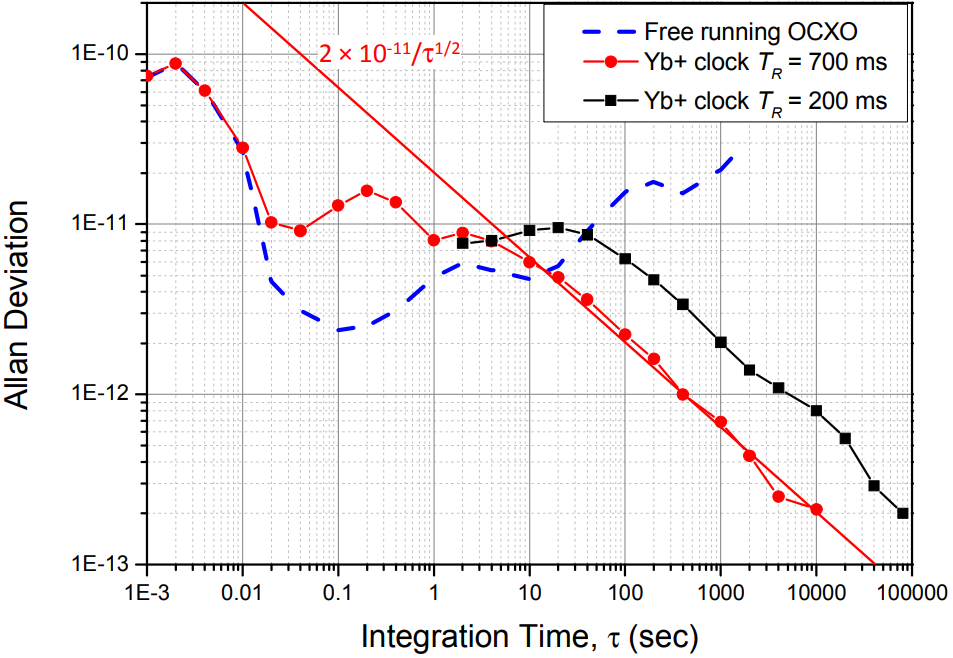
\includegraphics[height=0.4\textheight]{img/Ytterbium-stability.png}
                \caption{Sandia clock performances\footnotemark[1].}
            \end{figure}

        \end{column}

        \begin{column}{0.5\textwidth}

            \begin{figure}
                \centering
                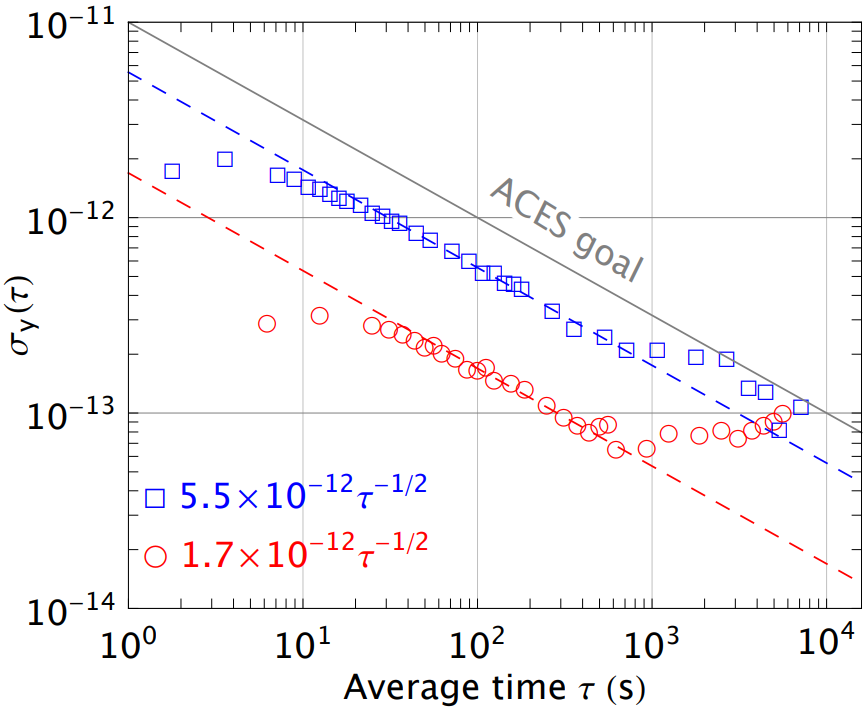
\includegraphics[height=0.4\textheight]{img/Mercury-stability.png}
                \caption{JPL clock performances\footnotemark[1].}
            \end{figure}

        \end{column}

    \end{columns}

    \vspace{10pt}

    \textbf{Trapped ions is probably the most promising solution for the NG-CSACs.}

    Further development is required to mitigate instabilities (Stark Shift effect) and reduce system complexity (pulsed laser interrogation).

    \footnotetext[1]{Performances are comparable recalling the different size of the two systems.}

\end{frame}
\section*{Optical transitions in warm atomic/molecular vapors}

\begin{frame}{Working principle}

    Large scale optical transitions clocks has already shown a short-term stability $\sigma_y(\tau = 1s) \approx 10^{-18}$.
    Here, \textbf{quartz crystal local oscillator is replaced by a laser tuned to an atomic transition}.

    \vspace{10pt}

    Two different physics are exploited to reduce the Doppler broadening:

    \begin{itemize}
        \item MTS\footnotemark[1]: nonlinear interaction of laser light with atoms allows the use of a dual laser system to enable sub-Doppler spectroscopy.
        \item TPS\footnotemark[2]: shift in frequency due to moving atoms are suppressed by using two laser waves travelling in opposite directions.
    \end{itemize}

    \footnotetext[1]{MTS: Modulation transfer spectroscopy}
    \footnotetext[2]{TPS: Two-photon transitions}

\end{frame}



\begin{frame}{Two-photon transitions based clocks}

    So far, just a few optical-CSACs have been developed (experimental stage) all exploiting TPS.

    \vspace{10pt}

    NIST Chip-Scale Optical Atomic Clock (2019).

    \begin{columns}[c, onlytextwidth]

        \begin{column}{0.65\textwidth}

            \begin{figure}
                \centering
                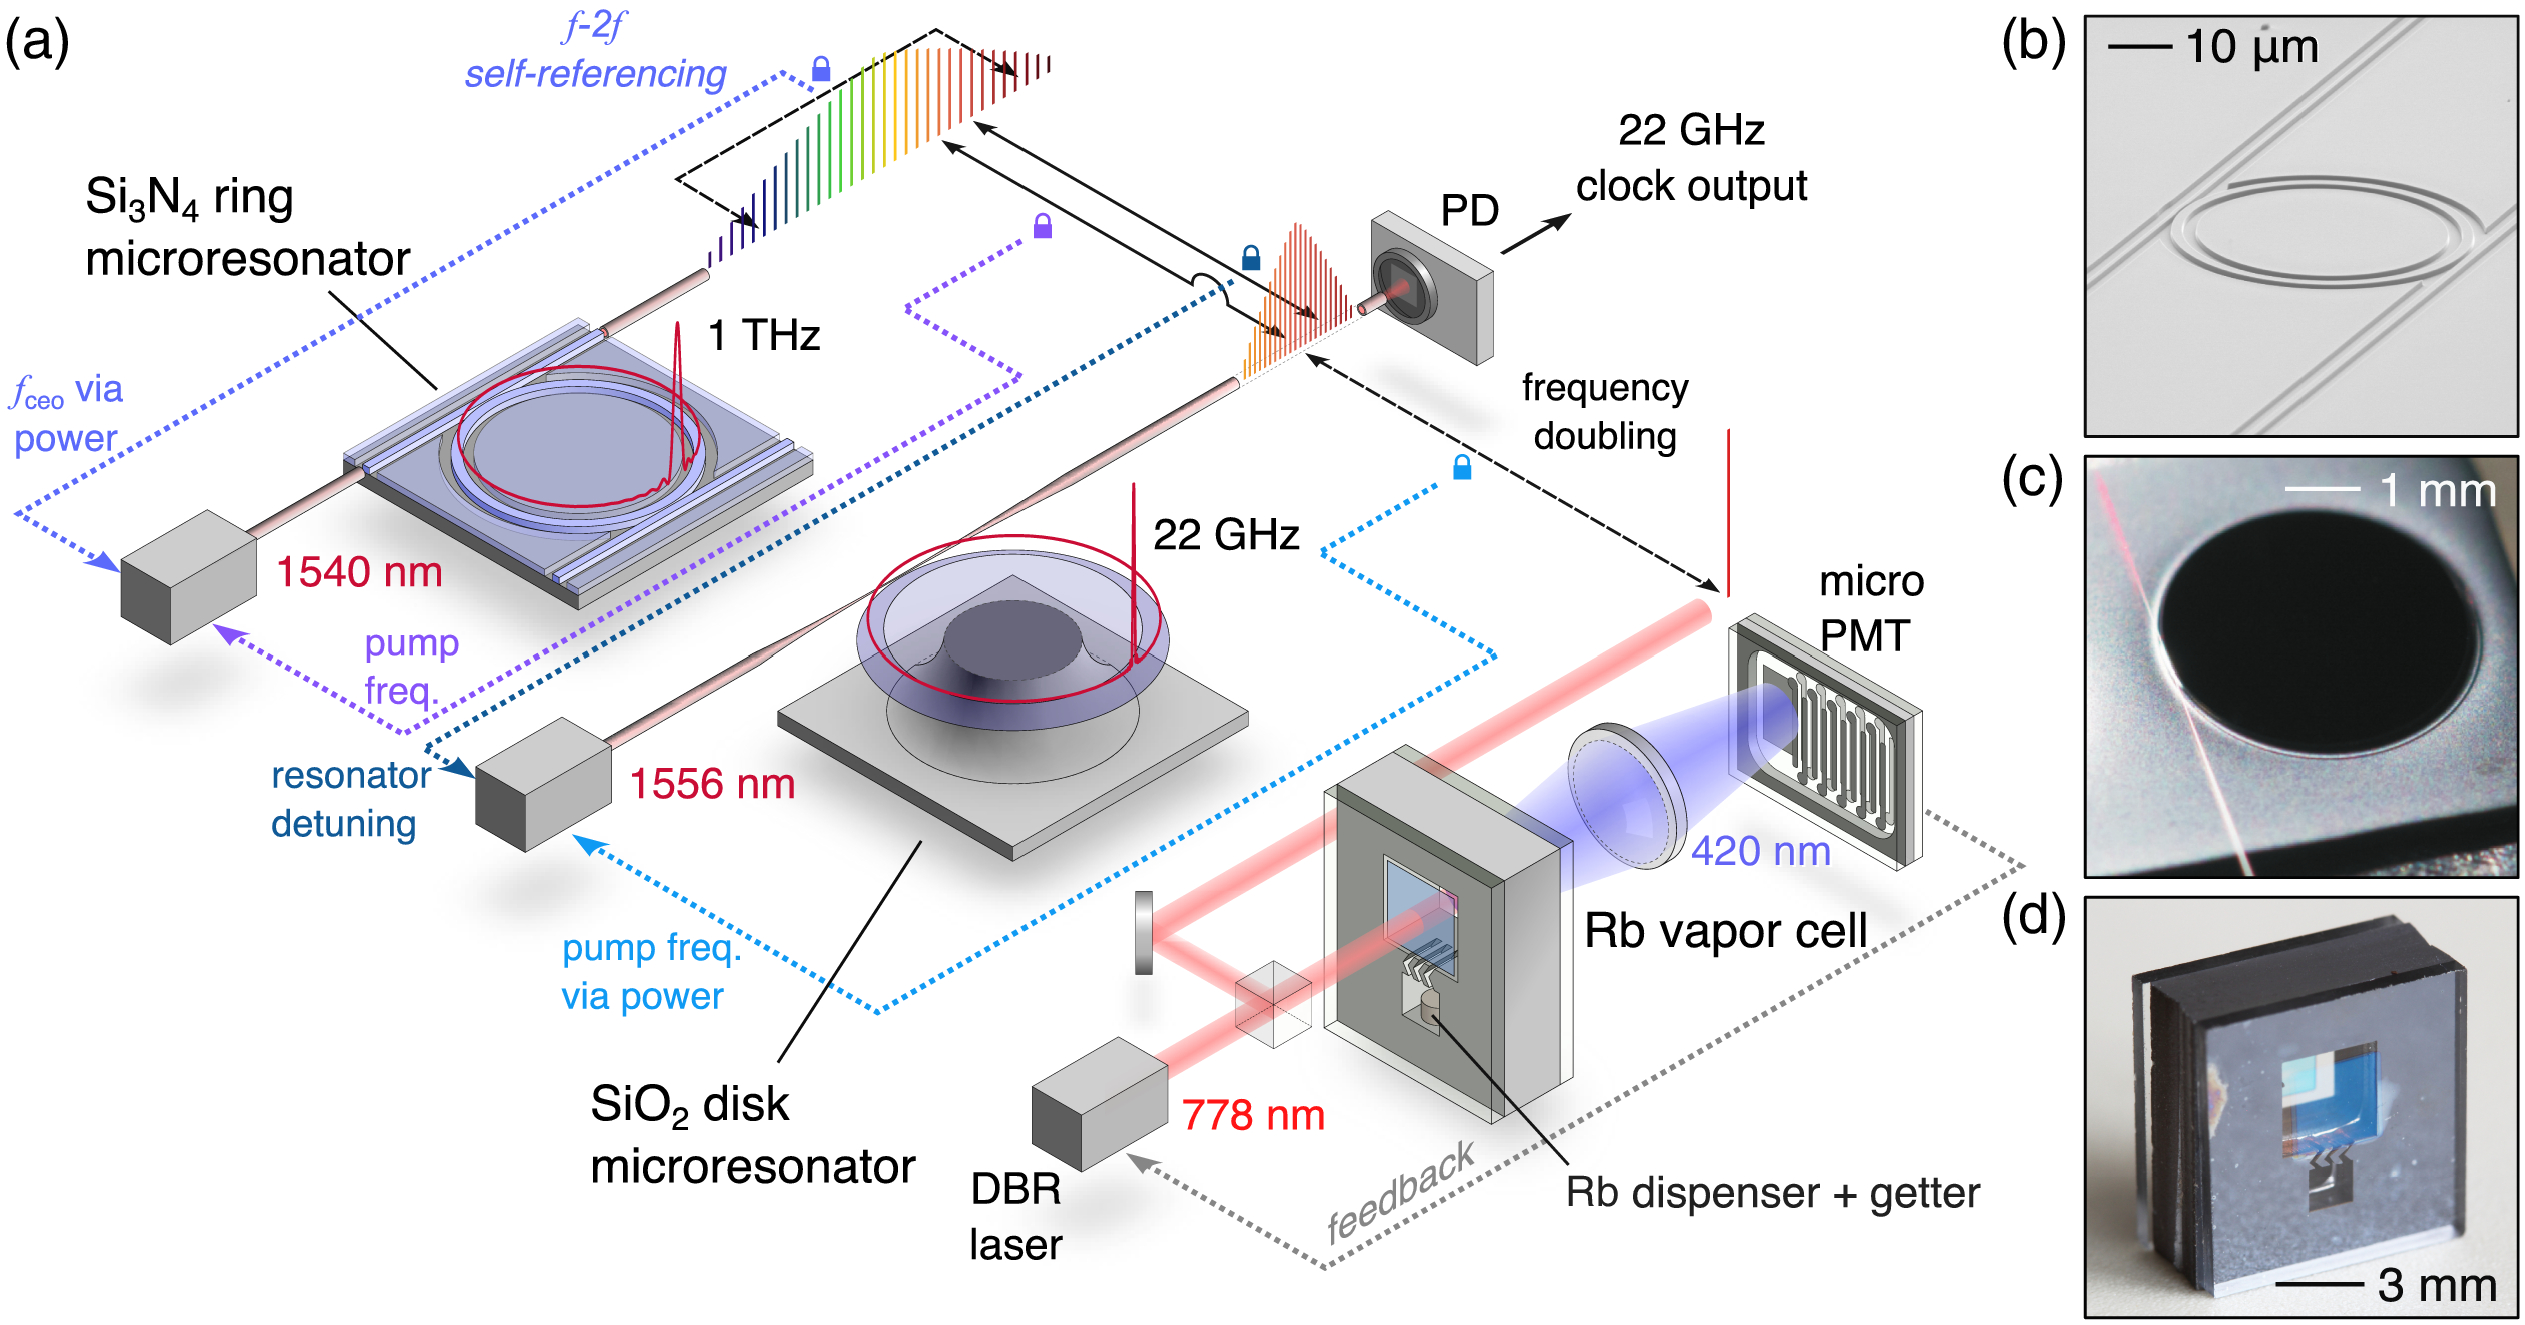
\includegraphics[width=\textwidth]{img/NIST-optical.jpeg}
            \end{figure}

        \end{column}

        \hfill

        \begin{column}{0.32\textwidth}

            Critical components:

            \begin{itemize}
                \item DBR\footnotemark[1] lasers
                \item Kerr-micro-resonator frequency combs
                \item Waveguides
            \end{itemize}

        \end{column}

    \end{columns}

    \vspace{10pt}

    The \textbf{miniaturization of all the required components is the main challenge} in the optics of the NG-CSACs.

    \footnotetext[1]{DBR: Distributed Bragg Reflector}

\end{frame}



\begin{frame}{Two-photon transitions based clocks}

    \begin{columns}[c, onlytextwidth]

        \begin{column}{0.5\textwidth}

            \begin{figure}
                \centering
                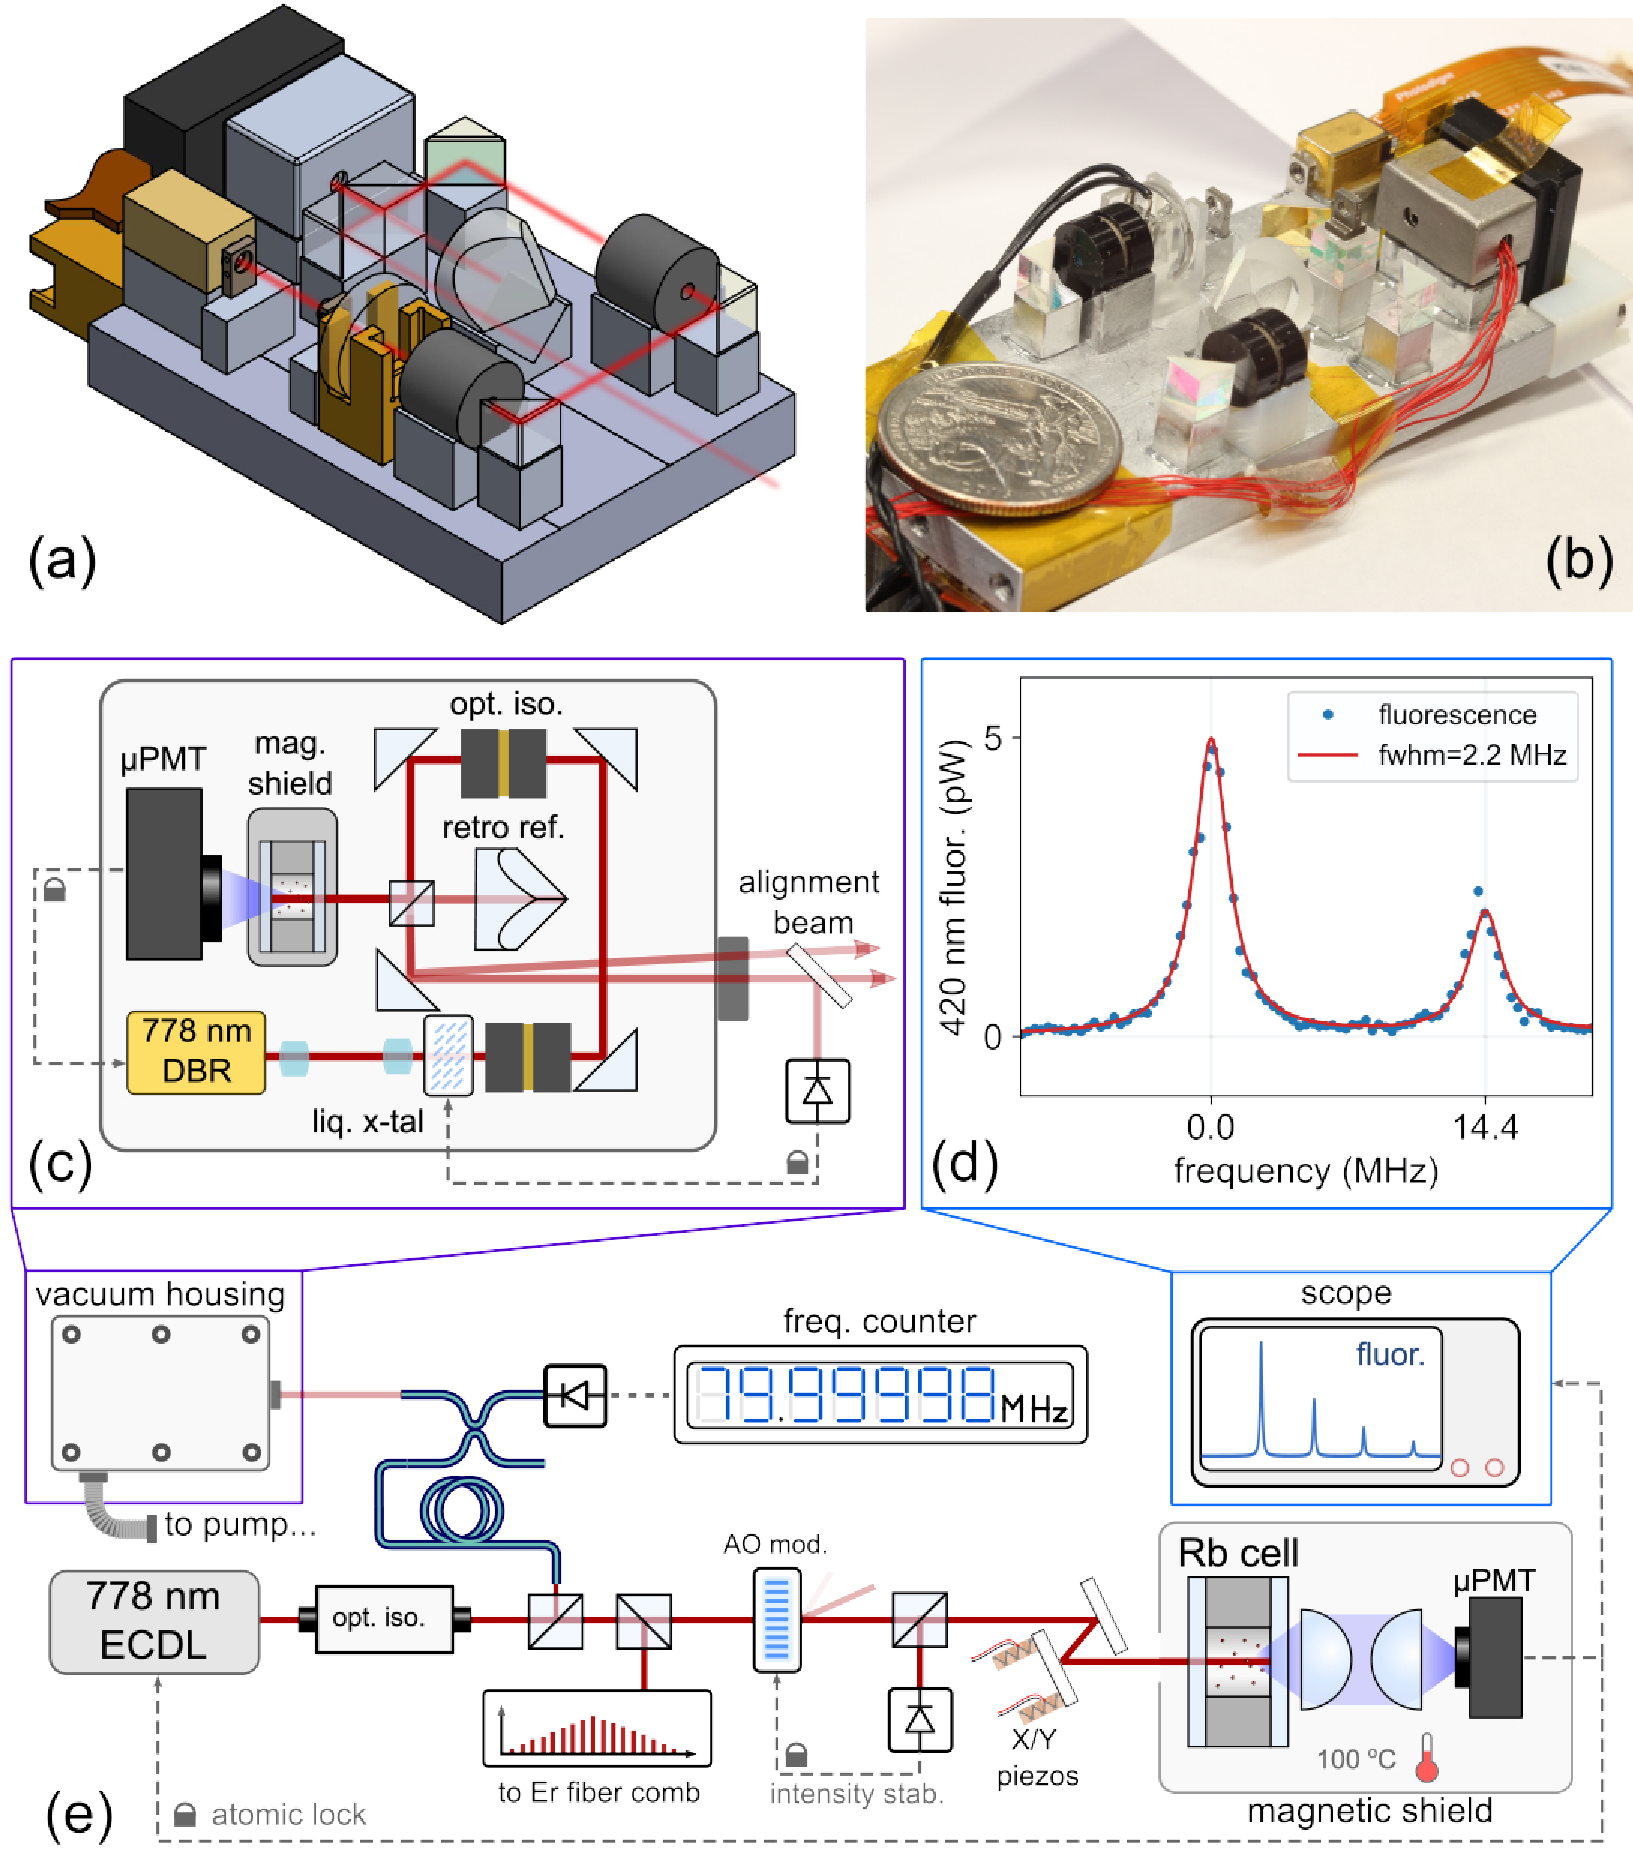
\includegraphics[width=\textwidth]{img/NIST-DRAPER-optical.jpeg}
            \end{figure}

        \end{column}

        \hfill

        \begin{column}{0.45\textwidth}

            NIST \& DRAPER optical-MAC\footnotemark[1] (2020).

            \vspace{10pt}

            Critical components:

            \begin{itemize}
                \item Microfabricated photomultiplier tubes
                \item DBR lasers
                \item Micro optics breadboards components
            \end{itemize}

        \end{column}

    \end{columns}

    \footnotetext[1]{MAC: Miniature Atomic Clock}

\end{frame}



\begin{frame}{Current results}

    Stability result shows that CSAC exploiting optical transitions met the DARPA ACES program requirements (shown in red in the figures below).

    \begin{columns}[T, onlytextwidth]

        \begin{column}{0.35\textwidth}

            \begin{figure}
                \centering
                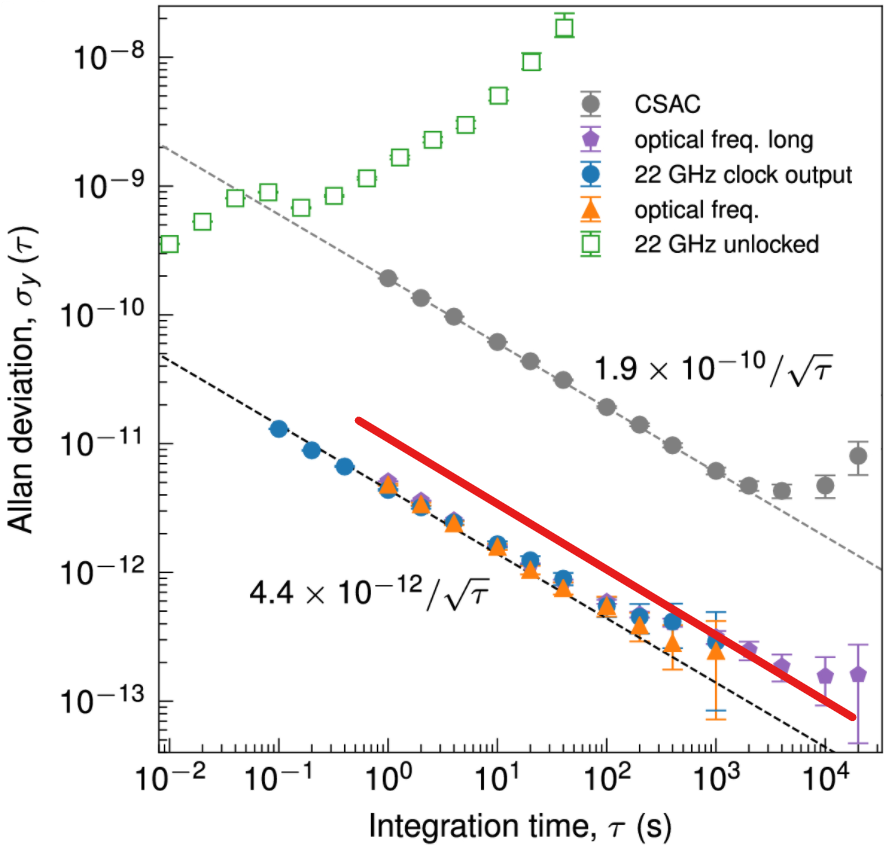
\includegraphics[width=\textwidth]{img/NIST-stability.png}
                \caption{NIST optical-CSAC stability.}
            \end{figure}

        \end{column}

        \hfill

        \begin{column}{0.55\textwidth}

            \begin{figure}
                \centering
                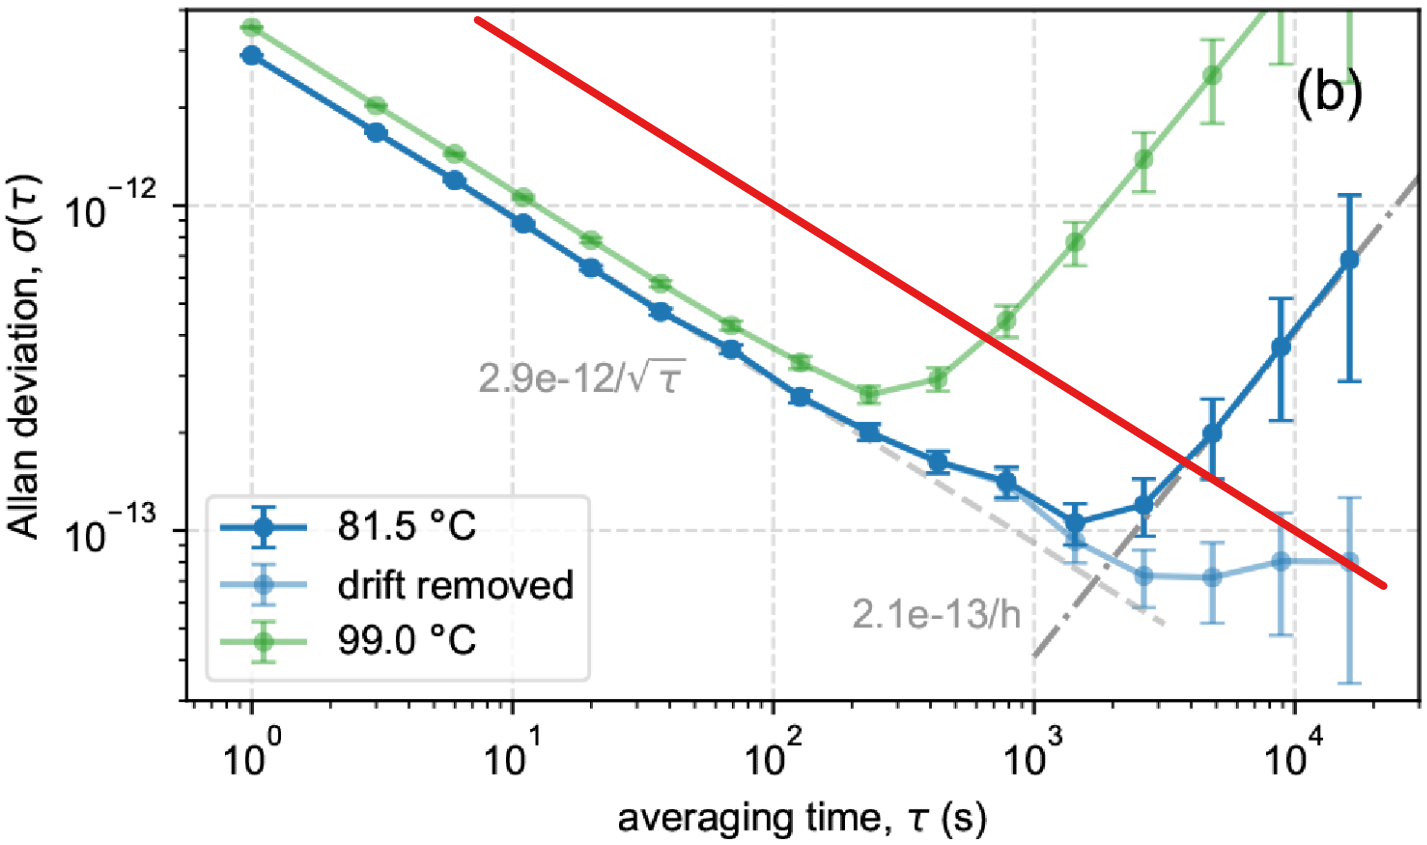
\includegraphics[width=\textwidth]{img/NIST-DRAPER-stability.png}
                \caption{NIST \& DRAPER optical-MAC stability.}
            \end{figure}
        \end{column}

    \end{columns}

    However, \textbf{the development of integrated custom micro components}, such as fast-frequency-tunable lasers and frequency microcombs, \textbf{is still a challenge}.

\end{frame}